\part{ÉTAT DE L’ART}
\chapter{PRÉSENTATION DU PROJET}

\textit{Dans ce premier chapitre de la première partie de notre mémoire, nous allons présenter
	notre projet, du contexte à la problématique, sans bien sûr oublier les méthodes. Il présente
	notre projet dans son ensemble, il présente la délimitation du sujet, les problèmes à résoudre,
	l’intérêt du sujet et une étude de l’existant.}

\clearpage

\section{Compréhension du sujet}

\subsection{Contexte}

L’apprentissage est un ensemble de mécanismes menant à l'acquisition de savoir-faire, de savoirs ou de connaissances afin de s’en servir dans la vie courante ou de les faire évoluer pour les générations futures.
Malgré les évolutions technologiques offrant de nouvelles façons d’acquérir des connaissances, le système éducatif africain, plus précisément camerounais n’a pas beaucoup évolué, les moyens de dispenser les connaissances ne suivent pas toujours les tendances actuelles.
Les personnes apprennent mieux en s’immergent dans ce qu’ils font qu’en le théorisant, cela est toujours possible dans le processus d’apprentissage, mais pas dans tous les domaines de formation du fait des risques lié à l’acquisition des connaissances en pratique.

Parmi ces domaines dans lesquels l’immersion réelle des apprenants dans les conditions réelles de pratique présente des risques réels pour l’apprenant, nous pouvons parler de la chimie, qui est un domaine de la science très expérimentale nécessitant des observations pour une compréhension du sujet étudié en vue d’y apporter des applications dans la vie courante.
Une grande et bonne compréhension de ce domaine pourrait apporter de nombreuses idées de recherche qui permettront des avancées significatives dans de nombreux domaines (agriculture, industrie, mode, la mécanique, l'énergie…), avancées qui pourraient à leur tour faciliter le processus d'émergence en Afrique et plus précisément au Cameroun.
Malgré l'aspect très expérimental de son apprentissage, il reste assez dangereux et couteux à enseigner en pratique, dangereux, car le manque d’expérience des apprenants pourrait les pousser à commettre des erreurs qui pourraient causer des accidents très dangereux, voire mortelle en fonction des éléments manipulés et couteux, car la maintenance du matériel nécessaire aux expérimentations (local, verrerie, éléments et personnelles de maintenance) engendre des coûts assez élevés.

\textbf{VREDU} est une plateforme dont l’objectif est de limiter les coûts et les risques lors des expérimentations en concevant le réalisme afin de créer un sentiment d’immersion pour une meilleure compréhension.
Pour ce faire, monglo technology s’est intéressé à la réalité virtuelle qui est une expression désignant les dispositifs permettant de simuler numériquement un environnement par la machine (ordinateur), afin d’apporter ce réalisme et limiter les risques d’accidents.

\subsection{Délimitation du sujet et hypothèse du travail}

Notre travail se limitera au cas des travaux pratiques de la chimie.

\begin{itemize}
	\item Création des réactions chimiques
	\item Expérimentation des réactions dans un environnement immersif
\end{itemize}

\section{Étude de l’existant}

L’étude de l’existant a pour but d'approfondir l'analyse des axes innovants d'un projet au cours d'élaboration, et avant sa mise en œuvre. Cette étude préalable sert à donner un aperçu sur la pertinence du projet, sa faisabilité ainsi que sa continuité.

\subsection{Description de l’existant}

Nous ne saurions commencer ce travail sans avoir une idée claire et précise sur l’existant quel qu’il soit.
Dans la plupart des lycées, l’enseignement de la chimie suit un modèle traditionnel, à savoir cours théoriques en salle de classe au cours duquel l’apprenant découvre les principes théoriques nécessaires à la maitrise de cette science. Ensuite, un cours pratique en laboratoire au cours duquel les apprenants découvrent la réalité des réactions grâce aux expériences scientifiques.


\subsection{Critique de l’existant et Problématique}

Au cours de notre étude de l’existant, nous avons pu ressortir de nombreux problèmes liés à la réalisation des réactions dans un environnement réel, parmi lesquelles :

\begin{itemize}
	\item Les risques d’accidents au cours d'expérimentation trop élevée dans un environnement réel, accident qui peut s’avérer mortel suivant les éléments manipulés.
	\item Les coûts de maintenance des équipements qui avec le temps se détériorent et nécessitent d’être renouvelé ou entretenu régulièrement ce qui entraine des couts matériels et humains assez importants.
\end{itemize}

Ceci nous a poussé à soulever la problématique : \textbf{\og \pb ? \fg} Autrement dit, pourrait–on envisager une plateforme permettant la simulation d’un laboratoire de chimie en limitant les risques d’accidents au cours des expérimentations et aussi en limitant les coûts de maintenance du matériel une fois l'environnement fonctionnel ?

\subsection{Quelques solutions existantes}

Il est question ici de noter les points forts de ces dernières et leurs points faibles afin d’ajuster nos objectifs.

\begin{itemize}
	\item \textbf{ONTOP DUO MEAC}

	      Ontop duo meac est une technique de simulation de vol utilisé dans les écoles d’aviation utilisé par les formateurs pour mettre en pratique les aspects théoriques abordés durant les formations. 
		  En effet, dans le domaine de l’aviation, les simulateurs de vol comme celui-ci sont presque incontournables, car en cas d’accident en condition réel dû au manque d’expérience des apprenants, les nombreuses vies seront menacées et des équipements très coûteux seront détruits.

	      Le dispositif est composé d'écrans disposés à 180° autour de l’apprenant afin de simuler le point de vue d’un pilote et d’un cockpit fidèle à leur homologue réel.

	      \begin{figure}[H]
		      \centering
		      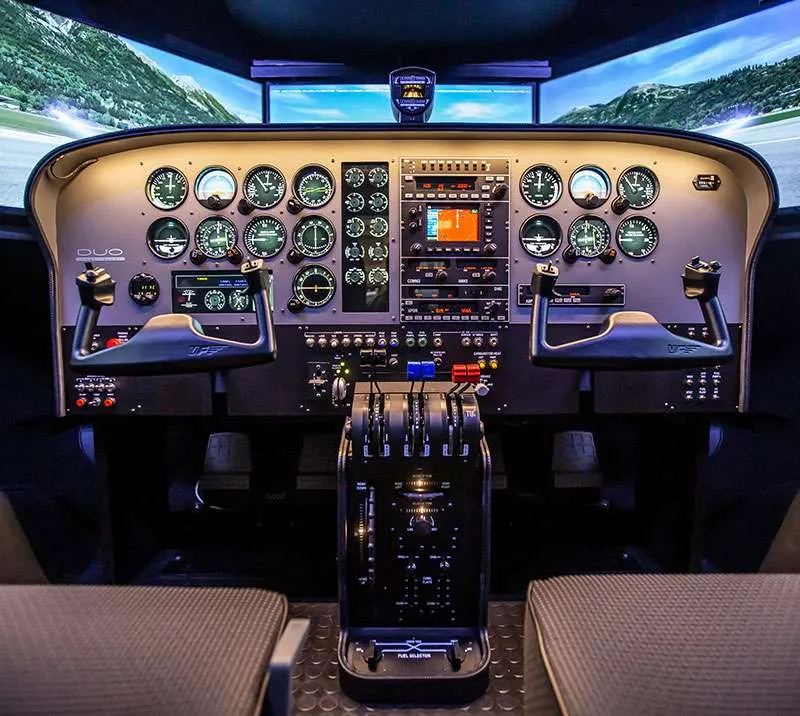
\includegraphics[width=0.5\textwidth]{img/svol1}
		      \caption{Simulateur de vol ONTOP DUO MEAC}
		      \label{fig:mesh1}
	      \end{figure}

	\item \textbf{Microsoft flight simulator}

	      Flight Simulator est un logiciel de simulation de vol pour Microsoft Windows, vendu et souvent vu comme un jeu vidéo. Tout comme l'Ontop duo meac, il permet à l'apprenant de comprendre le domaine de l’aviation en pratiquant à moindre coût car il n’a besoin que d’une console de jeux (PlayStation, Xbox, etc) et de contrôleurs, ici des manettes des consoles ou des dispositifs spéciaux.

	      Cette technique est beaucoup moins rependue dans les centres de formation, car elle est plus adaptée pour les apprenants désireux de s’entrainer chez eux et ne disposant pas des moyens pour un Ontop duo meac.

	      \begin{figure}[H]
		      \centering
		      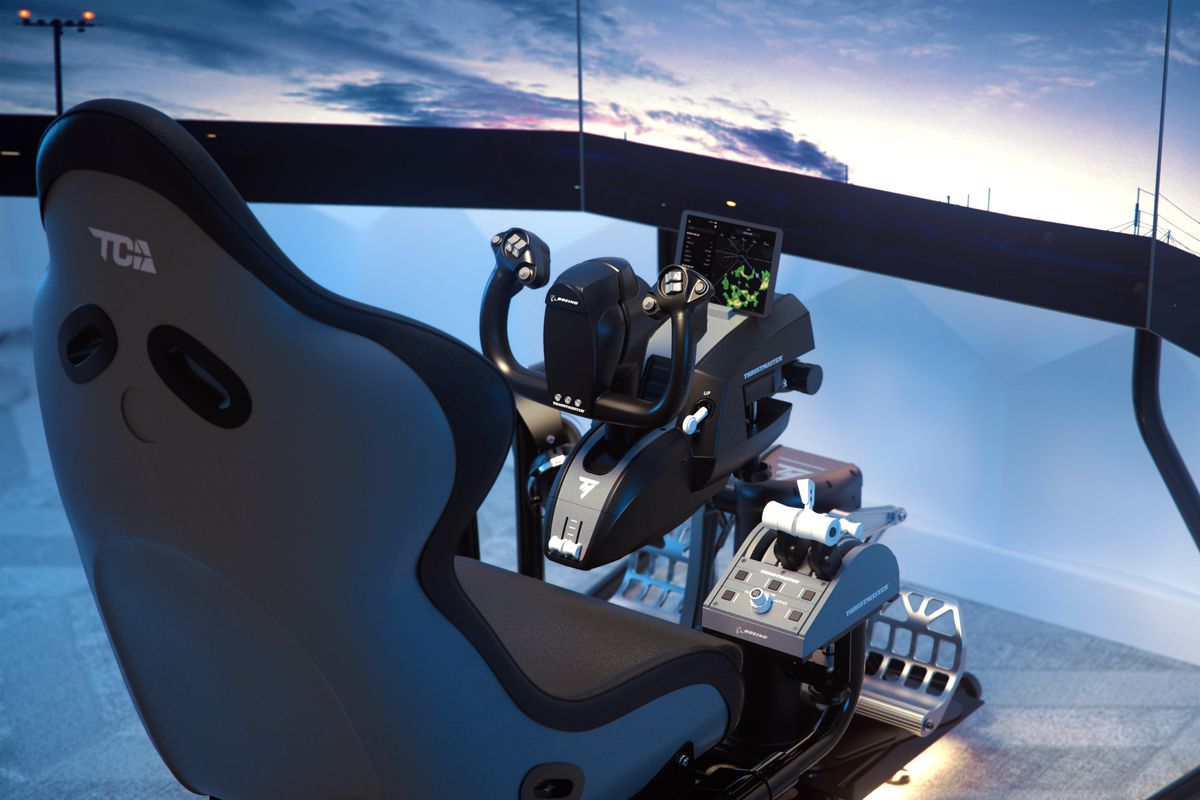
\includegraphics[width=0.5\textwidth]{img/svol2}
		      \caption{Simulateur de vol Microsoft flight simulator}
		      \label{fig:mesh1}
	      \end{figure}

	\item \textbf{Osso VR}

	      Osso VR est une plateforme de formation et d'évaluation chirurgicales qui offre aux entreprises de dispositifs médicaux et aux professionnels de la santé des moyens radicalement meilleurs de partager, de pratiquer. 
		  Tout comme dans le domaine de l’aviation, le domaine médical, plus précisément chirurgical utilise des outils de simulation de l’aspect pratique de l’apprentissage. 
		  Ceci dû aux risques liés à l’expérimentation sur des individus vivants et le manque de cadavre.

	      Osso VR utilise la réalité virtuelle pour les expérimentations, afin de simuler un monde en trois dimensions représentant un laboratoire dans lequel est disposé un patient virtuel sur lequel seront effectuées les expérimentations.

	      \begin{figure}[H]
		      \centering
		      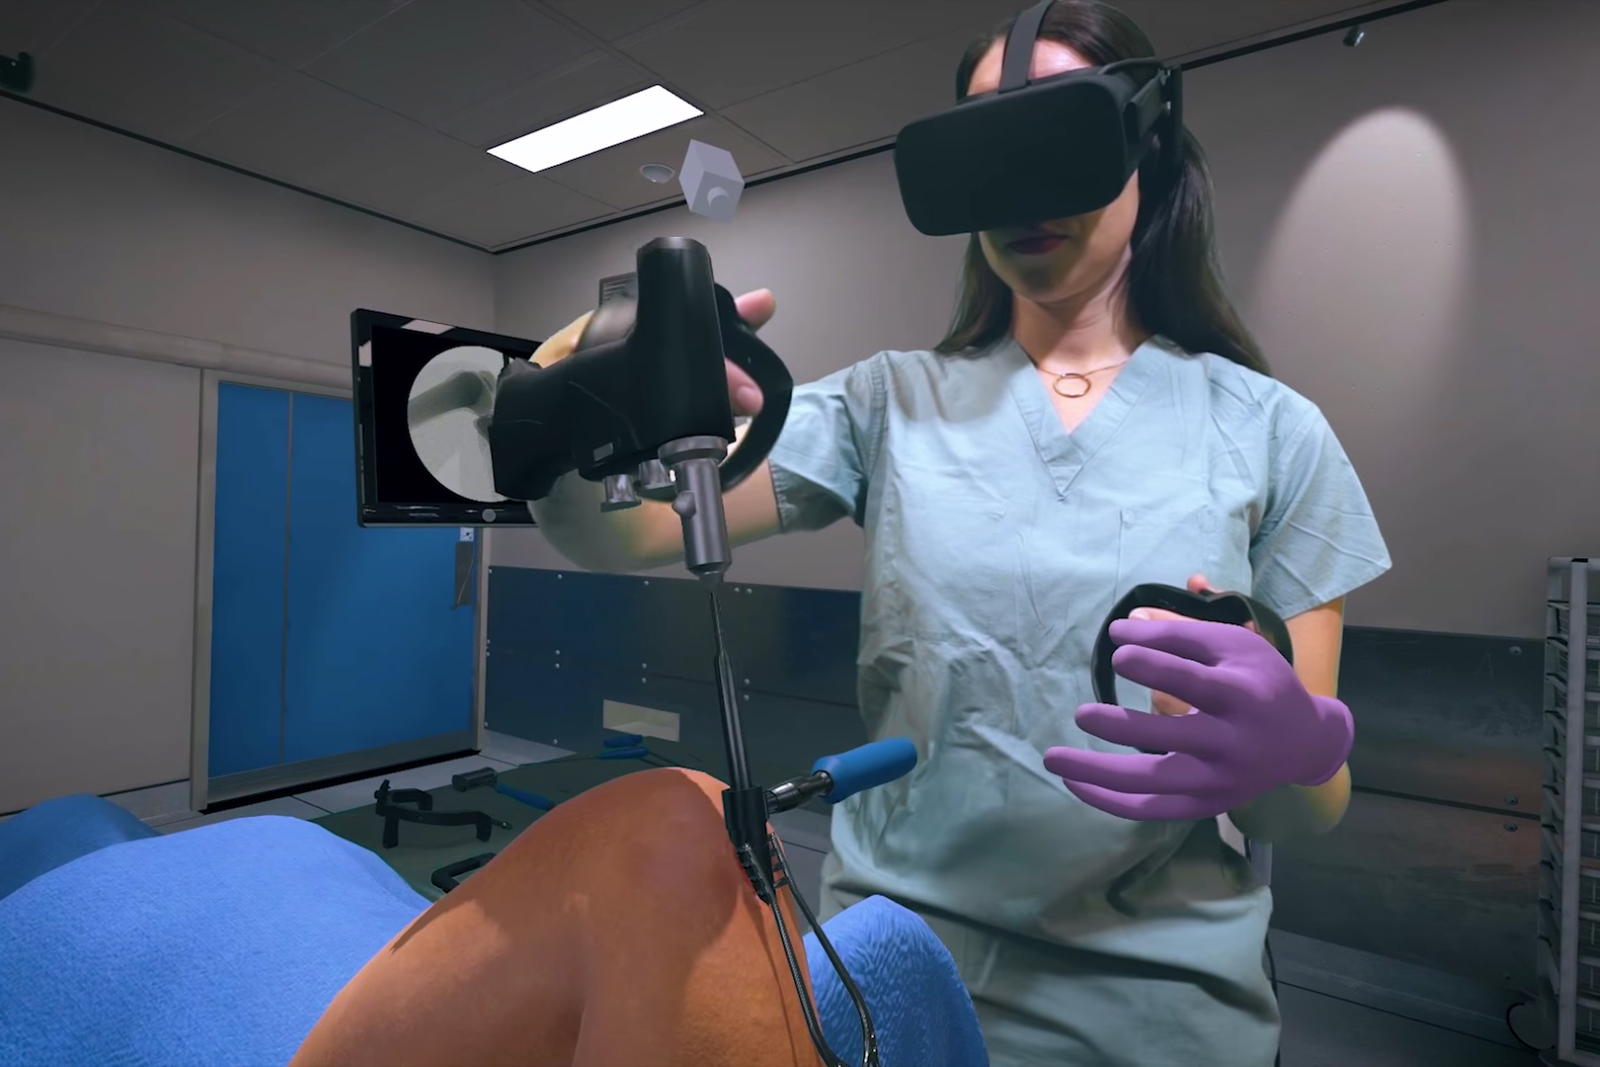
\includegraphics[width=0.5\textwidth]{img/vsurgery}
		      \caption{Simulateur chirurgical Osso VR}
		      \label{fig:mesh1}
	      \end{figure}

	\item \textbf{Praxilab}

	      Praxilab est un outil didacticiel permettant la simulation d'expériences scientifiques dans les domaines de la biologie, la physique et la chimie. 
		  Cet outil est développé pour les plateformes desktop et web.
		  Il permet aux apprenants de suivre des instructions afin de réaliser des expériences et comprendre des phénomènes liés aux différents domaines.

	      \begin{figure}[H]
		      \centering
		      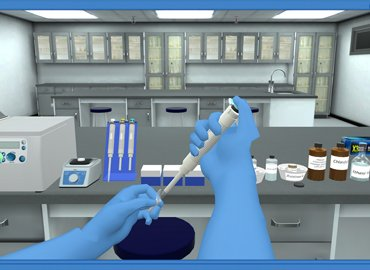
\includegraphics[width=0.5\textwidth]{img/vlab1}
		      \caption{Simulateur scientifique Praxilab}
		      \label{fig:mesh1}
	      \end{figure}

	\item \textbf{EON Reality}

	      EON Reality est une solution de formation académique et industrielle en réalité augmentée et virtuelle. 
		  Elle permet l'expérimentation virtuelle dans plusieurs domaines de l’enseignement, à savoir la mécanique, la chimie, la biologie, l’histoire, le génie civil et plein d’autres domaines.

	      Cette solution est disponible sur de nombreux supports à savoir ordinateur sur Windows, casques de réalité virtuelle oculus, sous Android et ios.

	      \begin{figure}[H]
		      \centering
		      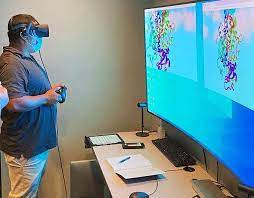
\includegraphics[width=0.5\textwidth]{img/vlab2}
		      \caption{Simulateur scientifique EON RealityC}
		      \label{fig:mesh1}
	      \end{figure}
\end{itemize}

\begin{table}[H]
	\centering
	\caption{Comparatif des solutions existantes}
	\begin{tabular}{|l|p{5cm}|p{5cm}|}
		\hline
		\textbf{Application}       & \textbf{Avantages}                                                                                      & \textbf{Inconvénants}                                                          \\ \hline
		ONTOP DUO MEAC             & Très immersif et très réaliste, maintenu et populaire dans le milieu de l'aviation.                          & Trop chère pour une utilisation à domicile, pas adapté aux sciences chimiques. \\ \hline
		Microsoft flight simulator & Assez peu chère à l'obtention donc adapté à une utilisation à domicile et maintenu                      & Pas très immersif et réaliste, pas adapté aux sciences chimiques                \\ \hline
		Osso VR                    & Immersif, assez réaliste et maintenu                                                                    & Disponible seulement en démo, pas adapté aux sciences chimiques.                \\ \hline
		Praxilab                   & Assez réaliste, accessible, adapté aux expérience chimiques et maintenu                                   & Pas très immersif, impossible de créer des réactions, pas de version française \\ \hline
		EON Reality                & Immersif, très polyvalent, disponible sur de nombreuses plateformes et en plusieurs langues, et maintenu & Impossible de créer des réactions                                              \\ \hline
	\end{tabular}
\end{table}

\subsection{Questions de recherche}

\begin{itemize}
	\item Comment pouvons-nous rendre l'enseignement de la chimie moins couteux ?
	\item Comment pouvons-nous rendre l'enseignement de la chimie moins risqué ?
	\item Comment conserver l'aspect réaliste et immersif des expérimentations réelles ?
	\item Comment permettre aux enseignants de créer des réactions pour leurs expérimentations ?
\end{itemize}

\section{Choix et intérêt du sujet}

Le contexte dans lequel nous nous trouvons et la problématique nous oriente vers un
choix de thème qui est \textbf{\og \theme \fg}.
La plateforme \textbf{VREDU Chemistry lab} permettra non seulement de résoudre le problème lié aux coûts de maintenance
du matériel et des infrastructures en limitant aussi les risques au cours des expérimentations.

\section{Objectif du travail}

L’objectif principal est d'apporter un outil d'aide à l'enseignement secondaire, plus précisément de la chimie afin qu'un enseignant puisse créer des réactions que les apprenants suivront durant la phase pratique du cours.

Les objectifs spécifiques sont :

\begin{itemize}
	\item Représentation des réactifs et des produits en trois dimensions et de façon réaliste et immersive
	\item Calcul de la quantité de matière des réactifs dans une solution
	\item Calcul de la concentration des réactifs dans une solution
	\item Calcul de la masse molaire moléculaire des réactifs dans une solution
	\item Calcul du ph d’une solution
\end{itemize}

\section{Méthodologie}

\subsection{Gestion de projet}

Pour le pilotage de notre projet, nous devons choisir parmi les méthodes de gestion de projets une qui convient le mieux non seulement à notre projet, mais également à notre contexte en entreprise.
Pour ce faire, nous allons dans un premier lieu faire une comparaison de ces
méthodes afin de faire un choix convenable.

Alors que les méthodes traditionnelles visent à traiter les différentes phases d’un projet d’une manière séquentielle (que l’on nomme aussi cycle de développement en cascade ou encore cycle
en V), le principe des méthodes Agiles est de le découper en sous-parties (ou sous-projets)
autonomes (on parle également de développement itératif). Les parties (itérations) forment le
projet dans sa globalité.

Nous allons présenter dans un tableau une étude comparative entre l’approche de gestion de projets agiles et celle traditionnelle.


\begin{table}[H]
	\centering
	\caption{Comparaison entre les approches traditionnelles et agiles}
	\label{tab:my-table}
	\begin{tabular}{|l|p{5cm}|p{6cm}|}
		\hline
		\textbf{Thème}      & \textbf{Approche traditionnelle}                                                                       & \textbf{Approche agile}                                                                                                                                              \\ \hline
		Cycle de vie        & En cascade ou en V, sans rétroactions possibles, phases séquentielles                                   & Itératif et incrémental                                                                                                                                              \\ \hline
		Planification       & Produite en quantité importante comme support de communication, de validation et de contractualisation & Réduite au strict nécessaire au profil d’incréments fonctionnels opérationnels pour le feedback du client                                                            \\ \hline
		Équipe              & Contrôle de qualité à la fin du cycle de développement. Le client découvre le produit fini.            & Un contrôle de qualité précoce et permanent au niveau du produit et du processus. Le client visualise les résultats tôt et fréquemment                               \\ \hline
		Qualité             & Une équipe avec des ressources spécialisées et dirigées par un chef de projet.                            & Une équipe responsabilisée ou l’initiative et la communication sont privilégiées et soutenues par le chef de projet                                                       \\ \hline
		Suivi d’avancement  & Mesure de la conformité aux plans initiaux. Analyse des écarts.                                        & Un seul indicateur d’avancement : le nombre de fonctionnalités implémentées et le travail restant à faire.                                                            \\ \hline
		Changement          & Résistance, voire opposition au changement. Processus lourd de gestion des changements acceptés          & Accueil favorable au changement, intègre dans le processus                                                                                                           \\ \hline
		Gestion des risques & Processus distinct, rigoureux de gestion des risques                                                    & Gestion de risques intégrée dans le processus global, avec responsabilisation de chacun dans l’identification et la résolution des risques. Pilotage par les risques \\ \hline
		Mesure du succès    & Respect des engagements initiaux en termes de coût, de budget et ce niveau de qualité                 & Satisfaction client par la livraison de valeur ajoutée                                                                                                               \\ \hline
	\end{tabular}
\end{table}

De cette comparaison, il est possible de choisir, selon le projet, l’approche qui convient le
mieux.

Au vu de notre projet, il convient pour nous de choisir une méthode agile, car cette dernière
s’adapte facilement aux changements et n’impose pas une planification rigide dès le début du
projet. Parmi les méthodes agiles existantes, nous devons en choisir une qui nous convient
encore plus. Après cette comparaison, notre choix s’oriente vers SCRUM.
Car au vu de la grandeur de notre projet, de la taille de l’équipe, des préférences de l’entreprise et de l’approche orientée objet, nous pensons qu’elle est la méthode la mieux adaptée.

\begin{table}[H]
	\centering
	\caption{Comparaison des méthodes agiles}
	\label{tab:my-table}
	\begin{tabular}{|l|l|l|l|}
		\hline
		\textbf{Méthode}                & \textbf{Flexibilité} & \textbf{Itératif} & \textbf{Taille} \\ \hline
		\textbf{Scrum}                  & oui                  & oui               & toute           \\ \hline
		\textbf{Crystal clear}          & oui                  & Non               & petite          \\ \hline
		\textbf{Processus unifié Agile} & oui                  & Non               & toute           \\ \hline
		\textbf{eXtreme Programing}     & oui                  & oui               & petite          \\ \hline
	\end{tabular}
\end{table}

\subsubsection{Qu’est-ce que la méthode SCRUM}

Scrum est un cadre léger qui aide les personnes, les équipes et les organisations à générer de la valeur grâce à
des solutions adaptatives pour des problèmes complexes\cite{schwaber2011scrum}.

Souvent considéré comme un framework de gestion de projets Agiles, Scrum décrit un ensemble de réunions, d'outils et de rôles qui interagissent de concert pour aider les équipes à structurer leur travail et à le gérer.

Scrum est fondé sur l'empirisme et la pensée Lean. L'empirisme affirme que la connaissance vient de l'expérience et de la prise de décisions basées sur ce qui est observé. La pensée Lean réduit le gaspillage et se concentre sur l'essentiel\cite{schwaber2011scrum}.

Scrum utilise une approche itérative et incrémentale pour optimiser la prévisibilité et contrôler les risques. Scrum engage des groupes de personnes qui ont collectivement toutes les compétences et l'expertise pour faire le travail et partager ou acquérir ses compétences selon les besoins. Scrum combine quatre événements formels pour l'inspection et l'adaptation dans un événement conteneur, le sprint. Ces événements fonctionnent parce qu'ils mettent en œuvre les piliers empiriques de Scrum que sont la transparence, l'inspection et l'adaptation.

\vspace{1em}
\begin{itemize}
	\setlength\itemsep{1em}
	\item \textbf{La transparence} : la transparence est un facteur clé de réussite. Tout au long du développement du produit, l’équipe de développement et les parties prenantes ont accès aux informations basées sur un langage et des définitions communs. Par exemple, la définition de fini (DOD, definition of done) est obligatoire et très importante pour Scrum. La définition de prêt (DOR, definition of ready) est aussi une pratique couramment utilisée, mais non obligatoire à ce jour si on se réfère au scrum guide.
	\item \textbf{L'inspection et l'adaptation} : l’équipe doit se consulter quotidiennement pour détecter rapidement d’éventuels écarts entre l’objectif de l’itération (Sprint Goal) et le travail réalisé. Cette Inspection dans le sprint a lieu principalement lors du Daily scrum, de la Sprint Review et de la Sprint Retrospective. Si des écarts sont constatés, un ajustement doit être entrepris afin d’atteindre les objectifs du sprint.

	      L’Inspection et l’adaptation permettent d’ajuster en permanence le développement d’un produit en fonction de l’apprentissage réalisé lors de chaque itération.
\end{itemize}

\subsubsection{Pourquoi la méthode SCRUM}

Cette méthode permet de répondre aux besoins des utilisateurs rapidement, dans les délais
impartis, tout en respectant les budgets. En effet, elle canalise et modélise toutes les étapes du
développement d’un logiciel. Elle ordonne aussi très clairement les différents jalons.

\subsubsection{Avantages de la méthode SCRUM}

Les équipes qui optent pour la structure Scrum gagnent en agilité et en flexibilité. Elle contribue à renforcer la collaboration au sein des équipes et les aide à atteindre leurs objectifs plus efficacement. Par ailleurs, les équipes Scrum savent en permanence sur quoi elles travaillent : elles accomplissent des tâches de leur backlog produit et ont une idée claire de leurs objectifs, car elles se sont concertées sur la définition d’un travail \og terminé\fg.

\subsubsection{Dans quels cas utiliser la méthode SCRUM}

Offrant plus de réactivité, elle est plus adaptée que les méthodes traditionnelles pour la gestion de projets web, tel que le développement logiciel, car elle traduit et organise les projets de façon simple, transparente et pragmatique.

Ce framework, ou cadre de travail, est utile quand :

\vspace{1em}
\begin{itemize}
	\setlength\itemsep{1em}
	\item L’ensemble d’un projet complexe ne peut être ni anticipé ni planifié entièrement.
	\item Son pilotage demande un minimum de flexibilité pour intégrer facilement des changements aux planifications initiales.
\end{itemize}

\subsubsection{Principale contrainte de la méthode SCRUM}

Les projets Scrum souffrent souvent de dérives des objectifs, car cette méthode accepte et encourage le changement. Cependant, il présente des risques d’itérer sans obtenir de résultats concrets si les changements sont trop nombreux ou que les retours clients sont discordants.

\subsection{Analyse et Modélisation}

Pour la réalisation du projet, nous allons procéder comme suit :

\vspace{1em}
\begin{itemize}
	\setlength\itemsep{1em}
	\item Séparation des différents modules à déployer
	\item Développer les différents en utilisant l'approche de développement orienté objet
	\item Déployer ces modules pour la production
\end{itemize}

\subsubsection{L’approche orientée objet}

L’approche orientée objet considère le logiciel comme une collection d’objets dissociés,
identifiés et définis par des propriétés. Une propriété est soit un attribut, soit une méthode.
La fonctionnalité du logiciel émerge alors de l’interaction entre les différents objets qui le
constituent. L’une des particularités de cette approche est qu’elle rapproche les données et
leurs traitements associés au sein d’un unique objet. Un objet est caractérisé par plusieurs
notions dont :

\vspace{1em}
\begin{itemize}
	\setlength\itemsep{1em}
	\item \textbf{L’identité} : l’objet possède une identité, qui permet de le distinguer des autres objets, indépendamment de son état. On construit généralement cette identité grâce à un identifiant
	      découlant naturellement du problème (par exemple une Banque pourra être repéré par un code,
	      un Encaissement par un numéro identifiant, etc.)
	\item \textbf{Les attributs} : il s’agit des données caractérisant l’objet. Ce sont des variables stockant des
	      informations sur l’état de l’objet.
	\item \textbf{Les méthodes} : les méthodes d’un objet caractérisent son comportement, c’est-à-dire l’ensemble
	      des actions (appelées opérations) que l’objet est à même de réaliser. Ces opérations permettent
	      de faire réagir l’objet aux sollicitations extérieures (ou d’agir sur les autres objets). De plus, les
	      méthodes sont étroitement liées aux attributs, car leurs actions peuvent dépendre des valeurs
	      des attributs, ou bien les modifier.
\end{itemize}

La difficulté de cette modélisation réside dans la création d’une représentation abstraite, sous
forme d’objets, d’entités ayant une existence matérielle (Exemple : Banque, Guichet, Caisse, etc.) ou bien virtuelle (Exemple : Encaissement, Décaissement, Transfert de fonds, etc.).
La Conception Orientée Objet (COO) est la méthode qui conduit à des architectures logicielles
fondées sur les objets du système, plutôt que sur la fonction qu’il est censé réaliser.

\subsubsection{UML et MERISE}

Les différences entre l’approche objet avec UML et l’approche systémique (fonctionnelle)
avec Merise sont mises en évidence dans l’étude comparative ci- dessous :

\vspace{1em}
\begin{itemize}
	\setlength\itemsep{1em}
	\item \textbf{Points communs} :

	      L’approche classique et l’approche objet distinguent bien globalement trois grandes étapes dans le processus de conception et de développement d’une solution : l’analyse objet correspond au niveau conceptuel de merise, la conception objet est proche de la modélisation logique et organisationnelle de merise. 
		  Et enfin l’implémentation objet correspond à la réalisation dans merise.

	      Nous allons reprendre chaque grand niveau de représentation du SI et donner un certain nombre
	      de précisions sur les points communs.

	      Le niveau de l’analyse objet ou le niveau conceptuel : dans les deux approches, la finalité de ses premiers niveaux de description d’un SI est d’appréhender les besoins à satisfaire et à donner une description de solutions indépendamment des considérations techniques des niveaux logiciels et physiques. Autrement dit, les préoccupations traitées sont très proches malgré des concepts par complètements identiques au niveau conceptuel et au niveau de l’analyse objet.

	      Le niveau conception objet ou le niveau logique organisationnel : ce niveau de description a bien pour finalité dans les deux approches de représenter la solution à implémenter sous l’angle de la logique informatique tant sur la partie des données que sur celle des traitements. Le niveau implémentation physique ou opérationnel dans les deux approches la préoccupation est la description physique et opérationnelle des données et des traitements.

	\item \textbf{Différences} :

	      Nous observons les différences entre ces deux approches au niveau des domaines d’application,
	      de la démarche, les données et les traitements puis l’aspect évolution du système.

	\item \textbf{Les domaines d’application} :

	      Merise a pour vocation de traiter les systèmes d’information des entreprises, principalement dans le domaine de l’informatique de gestion. Le domaine de l’informatique de gestion se caractérise en général par un grand nombre de données à gérer et à stocker avec des traitements relativement peu complexes.

	      Le domaine privilégié par UML est le domaine de l’informatique technique ou industrielle caractérisé par la gestion de composants physiques du monde réel (Informatisation des automates est représentative de ce domaine). 
		  Dans ce type de domaine, les aspects traitements d’états et comportements des objets, prennent le pas sur la gestion des données. 
		  En plus de cet atout, UML traite également sans difficulté majeure le domaine tel que l’informatique de gestion.

	\item \textbf{La démarche}

	      Avec merise, la démarche est structurée en étapes et phases dont l’étude préalable, l’étude
	      détaillée, la réalisation et la mise en œuvre. Il correspond en effet au cycle de vie d’un système
	      d’information. Et l’ensemble des résultats produits à chaque étape constitue le cycle de décision.
	      Merise propose donc une démarche en cascade, c’est-à-dire qu’une étape ne peut être entamée
	      que si l’étape précédente est achevée. Cela nécessite une organisation minutieuse du projet.
	      Dans le cas contraire, l’on pourrait noter quelques blocages ou une lenteur dans le processus
	      de modélisation du système d’information. Avec UML, la démarche est itérative, incrémentale,
	      guidée par les besoins des utilisateurs du système, et centrée sur l’architecture logicielle. La
	      démarche itérative permet de mieux comprendre et représenter un système complexe. Le
	      périmètre du système à modéliser est défini par les besoins des utilisateurs (les utilisateurs
	      définissent ce que doit être le système).

	\item \textbf{Choix d’une méthode d’analyse}

	      Suite à notre étude comparative entre l’approche systémique avec Merise et l’approche objet avec UML, Nous opterons donc pour une méthode d’analyse suivant l’approche objet dont UML pour la modélisation, dans l’étude conceptuelle de notre système.
	      Ensuite, au vu des circonstances et les délais de notre projet, nous optons pour une démarche itérative, incrémentale, guidée par
	      les besoins des utilisateurs du système. De plus, nous souhaiterions organiser nos programmes
	      en rassemblant les données et les traitements en vue de former des entités cohérentes, logiques
	      et stables. Enfin, nous aimerions faciliter les éventuelles évolutions et maintenances du système.
\end{itemize}

% \subsection{Langages et outils}

% \subsubsection{Choix du langage}


\chapter{GÉNÉRALITÉS SUR LES OUTILS D'APPRENTISSAGE IMMERSIF BASÉ SUR LA RÉALITÉ VIRTUELLE}


\textit{Afin de mener à bien un projet, il est important de comprendre les termes techniques tournant autour du sujet, notre thème porte ainsi sur la réalisation d'un outil d'apprentissage immersif basé sur la réalité virtuelle. Nous allons donc dans ce chapitre expliquer des concepts clés tels que l'apprentissage immersif et la réalité virtuelle}
\clearpage

\section{Apprentissage}

L'apprentissage a été défini fonctionnellement comme des changements de comportement qui résultent de l'expérience ou mécaniquement comme des changements dans l'organisme qui résultent de l'expérience\cite{deHouwer2013WhatIL}.
C'est le processus par lequel les êtres vivants acquièrent et transmettent leurs savoirs.
L'apprentissage a été un sujet central dans la recherche psychologique pratiquement depuis le début de la psychologie
en tant que science indépendante (par exemple, Ebbinghaus, 1885/1962 ; Thorndike, 1911).
Pendant la plus grande partie du siècle précédent, c'était même le sujet le plus étudié en psychologie.
De plus, aujourd'hui, les questions sur l'apprentissage sont abordées dans pratiquement tous les domaines de la psychologie et aussi de l'éducation\cite{deHouwer2013WhatIL}.
De sa définition ressort un principe important, celui de l'expérience, la répétition d'une action qui nous amène à mieux la comprendre.
L'acquisition de cette expérience est le principal défi auquel les organismes éducatifs doivent faire face aux vues du nombre grandissant de techniques et de moyen d'enseignant qui existe, moyens de plus en plus nombreux avec
l'essor des nouvelles technologies telle que le web.

Comme énoncé ci-dessus, il existe un grand nombre de techniques permettant de dispenser ou d'acquérir des connaissances par le moyen de l'apprentissage, parmi lesquelles les plus communément rencontrés sont l'apprentissage traditionnel et l'apprentissage par les jeux.

\subsection{L'apprentissage traditionnel}

Par apprentissage traditionnel, on entend le processus d'apprentissage moderne le plus répandu et le plus ancien qui consiste à dispenser des notions dans un cadre très académique et très strict qui ne laisse donc que peu de liberté d'action ou d'interprétation en limitant toute forme de distraction pour une concentration optimale afin
d'acquérir le maximum de connaissances sur un sujet en un temps données. Bien qu'assez ancienne comme méthode d'enseignement, elle tend à s'adapter à l'époque et aux contraintes auxquelles le monde est soumis notamment par sa digitalisation due aux avancées des TIC et à la récente pandémie de la covid qui ont créé un bouleversement dans son histoire, si bien que des écoles ou des formations
complètements digitalisées ont vu le jour et offrent des diplômes qui ne présentent aucune distinction de valeur par rapport à ceux obtenus en présentiel. Cela s'explique par le fait que ces deux modes d'études sont considérés comme parfaitement égaux et qu'aucune distinction n'est faite entre eux en matière d'emploi\cite{radovic2010advantages}.

Cette méthode d'apprentissage peut s'avérer très efficace pour l'apprentissage des petits enfants, mais des recherches récentes suggèrent que davantage de méthodes basées sur la découverte pourraient être encore plus efficaces.\cite{Weisberg2018GuidedPlay}

\subsection{L'apprentissage par le jeu}

L'apprentissage par le jeu est une approche pédagogique qui favorise le recours à des activités
ludiques pour stimuler de nombreux aspects du développement et de l'apprentissage de l'enfant\cite{AngelaPyle2018Apprentissage}.
Au début des années 2000, il y a eu un basculement vers la recommandation de l’emploi de
l’apprentissage par le jeu dans les programmes éducatifs préscolaires dans plusieurs pays,
notamment le Canada,\cite{whitebread2009play}
la Suède,\cite{Daubert2018Play}
la Chine,\cite{pyle2017continuum}
les Émirats arabes unis\cite{Hassinger2018Playing}
et la Nouvelle-Zélande\cite{Daubert2018Play}. L'environnement moins académique et moins strict permet aux apprenants de réellement explorer
le sujet soit de manière complètement autonome grâce aux jeux libre\cite{Berk2018Role} dirigé par l'enfant lui-même, soit avec un degré d'encadrement grâce aux jeux dirigés\cite{Bergen2018Cognitive}.

Ce type d'apprentissage est plus ou moins efficace en fonction de l'expérience immersive que propose. En effet, l'opposition des méthodes d'apprentissage par le jeu immersive et non immersive a montré qu'un apprenant aura beaucoup plus de facilité à comprendre un sujet et à s'y intéresser davantage lorsqu'il y est complètement immergé\cite{de2017motivational,Shackelford2019RelationshipsBC,Abdelaziz2020TheIO}.

\section{La réalité virtuelle et l'éducation}
\subsection{La réalité virtuelle}

Le virtuel peut être défini comme \og étant par essence ou effet, mais pas en fait \fg\cite{Jerald2015WhatIV} et la réalité comme \og l'état ou la qualité d'être réel \fg\cite{Jerald2015WhatIV}.
De la combinaison de ces deux concepts est né un environnement généré par ordinateur avec lequel il est possible d'interagir et de faire l'expérience des sens humains ordinaires comme si l'environnement était réel\cite{Rheingold1991VirtualR}.
La réalité virtuelle (VR) utilise des combinaisons de matériel informatique et de logiciels pour représenter différents aspects du monde physique à un individu en temps réel.
Un objectif clé de la conception de la réalité virtuelle est d'instiller un sentiment de présence, ou l'illusion d'être immergé dans l'environnement, par opposition à la simple visualisation de l'environnement d'un point de vue extérieur (voir illustration).

\subsubsection{Principe de fonctionnement}

Cinquante ans se sont écoulés depuis que Sutherland a présenté sa vision de l'Ultimate Display\cite{sutherland1965ultimate} imitant le monde réel dans tous les sens disponibles.
Et depuis lors, une grande quantité de technologies individuelles prenant en charge cette stimulation sensorielle ont émergé, mais ce n'est qu'en 1989 que Jaron Lanier a inventé le terme de réalité virtuelle\cite{Rheingold1991VirtualR}.
En 2012, près d'un quart de siècle après la première vague de réalité virtuelle, un projet Kickstarter nommé Oculus Rift, dans le but de fournir au public un écran monté sur la tête abordable et de haute qualité, cherchait un financement et a atteint l'objectif. de 250 000 \$ en moins de 24 heures. Ce fut l'étincelle initiale qui a lancé la deuxième vague de VR\cite{anthes2016state}.
La réalité virtuelle comme tous les domaines des TIC utilisent des périphériques de deux types, à savoir périphériques d'entrée et périphériques de sortie.

Les périphériques d'entrées en réalité virtuelles sont des équipements permettant à l'utilisateur d'interagir avec l'environnement 3D.
Le développement de ces périphériques est très diversifié et remplisse de nombreuses catégories parmi lesquelles nous pouvons citer des casques de réalité virtuelle, des contrôleurs ou manette de réalité virtuelle, des tapis roulant omnidirectionnel, des capteurs de posture, capteur de suivi des gestes\cite{anthes2016state}.

\textbf{Les casques de réalité virtuelle} : est le périphérique de sortie dans l'univers de la réalité virtuel, il permet la visualisation d'environnement 3D grâce à deux écrans disposés comme des lunettes au niveau des yeux de l'utilisateur et de capteur de mouvement permettant à l'utilisation d'un mouvement de tête de changer de point de vue dans l'environnement 3D.
De nombreux équipements l'affiche d'environnement en 3D ont vu le jour ces dernières années parmi lesquelles les plus connus sont : le rift d'oculus, le HTC Vive et le PlayStation VR.

\begin{figure}[H]
	\centering
	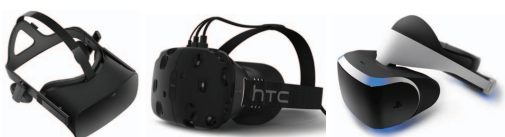
\includegraphics[width=0.5\textwidth]{img/3dcs}
	\caption{L'oculus rift (gauche), le HTC Vive (centre) et le PlayStation VR (droite) }
\end{figure}

\textbf{Les contrôleurs ou manette de réalité virtuelle,} ces équipements sont très proches des manettes traditionnelles utilisées pour des consoles de jeux telles que PlayStation et Xbox mais elles sont plus adaptées à un environnement immersif du fait de leur forme et du positionnement des boutons et des joysticks.
De nombreuses entreprises se sont lancées dans la conception de ces équipements parmi lesquelles nous pouvons citer : l'oculus Half Moon contrôleurs pour des casques de réalité virtuelle de la marque oculus, le steamVR pour le casque HTC Vive et Reactive Grip utilisable sur plusieurs marques de cas de réalité virtuelle parmi lesquelles oculus est vive.

\begin{figure}[H]
	\centering
	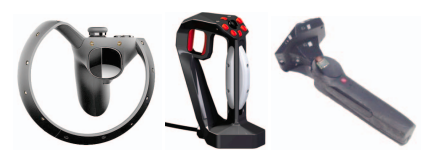
\includegraphics[width=0.5\textwidth]{img/3dcon}
	\caption{L'oculus Half Moon (gauche), le reactive Grip (centre) et le SteamVR (droite) }
\end{figure}

\textbf{Les tapis roulant omnidirectionnel} ce sont des équipements permettant le déplacement dans un environnement 3D en reproduisant les mouvements du monde réel, à savoir la marche, la course et les sauts grâce à un tapis roulant multidirectionnel auquel est attaché le sujet grâce à un harnais afin de suivre et de reproduire ses mouvements.
De nombreux équipements permettant la capture de ses différents mouvements existent parmi lesquelles nous avons : le Space Walker, le walkmouse et l'InfinaDeck.

\begin{figure}[H]
	\centering
	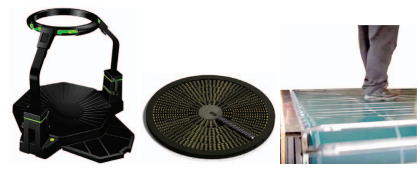
\includegraphics[width=0.5\textwidth]{img/3dtap}
	\caption{Le Virtuix Omni (gauche), le WalkMouse (centre), et le InfinaDeck (droite)}
\end{figure}

\textbf{Les capteurs de posture} ce sont des équipements permettant de reproduire les mouvements du squelette du sujet afin de le reproduire dans l'environnement. Ce type d'équipement créé un sentiment d'immersion dû à une reproduction des mimiques des utilisateurs.
De nombreux équipements permettant la capture de ses différents mouvements existent parmi lesquelles nous avons : le STEM, le PrioVR et ControllVR.

\begin{figure}[H]
	\centering
	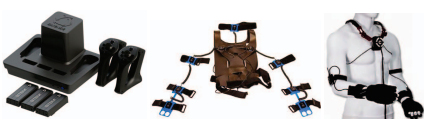
\includegraphics[width=0.5\textwidth]{img/3dcptt}
	\caption{Le STEM (gauche), le PrioVR (centre), et le ControllVR (droite)}
\end{figure}

\textbf{Les capteurs de suivi des gestes} permettant de capturer le mouvement des mains, ils viennent souvent remplacer les contrôler classiques, car moins immersifs et sont souvent utilisés avec le capteur de posture.
De nombreux équipements permettant la capture de ses différents mouvements existent parmi lesquelles nous avons : le Leap Motion, le Myo et le Glove One.

\begin{figure}[H]
	\centering
	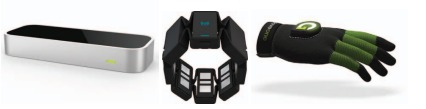
\includegraphics[width=0.5\textwidth]{img/3dgan}
	\caption{Le Leap Motion (gauche), le Myo (centre), et le Glove One (droite)}
\end{figure}

\subsection{La réalité virtuelle et l'éducation}

La réalité virtuelle n'est pas une nouvelle technologie. Mais, plusieurs contraintes ont empêché son adoption effective. Les progrès technologiques récents ajoutés à la prolifération de matériel et de logiciels abordables ont rendu la réalité virtuelle plus viable et souhaitable dans de nombreux domaines, notamment l'éducation; ils ont été relancés avec de nouvelles promesses jusqu'alors inimaginables. La nature de la réalité virtuelle promet de nouveaux modèles d'enseignement et d'apprentissage qui répondent mieux aux besoins de l'apprenant du 21e siècle.
Nous sommes maintenant sur la voie de réinventer l'éducation.

Cette technologie permet désormais d'enseigner en toute sécurité sans risque d'impact réel dans de nombreux domaines d'enseignement telle que la chimie, la biologie, la médecine et bien des domaines ou l'expérimentation est risquée soit pour l'apprenant ou son environnement.

Au cours d'une expérience dans un lycée chinois, lorsque du benzène a été ajouté à un mélange d'acide sulfurique concentré et d'acide nitrique concentré, le mélange s'est soudainement envolé du tube à essai et a éclaboussé les yeux de l'élève impliqué\cite{duan2020mixed}.
Les enseignants et les manuels expliquent très bien les risques liés à ce genre de réaction, mais en raison de leur manque de familiarité avec les procédures expérimentales sûres, les étudiants peuvent oublier les risques pour la sécurité lors de la réalisation d'une expérience\cite{duan2020mixed}.
Ces accidents surviennent également dans les établissements d'enseignement supérieur, comme les universités. Un accident récent s'est produit à l'Université Jiaotong de Pékin qui a causé la mort de trois étudiants qui participaient à l'expérience.
Allant de ce constat Xiaoyun Duan\cite{duan2020mixed} et une équipe de chercheur ont opté pour un dispositif utilisant la réaliter mixte\footnote{La réalité mixte est la fusion de mondes réels et virtuels pour produire de nouveaux environnements et visualisations, où les objets physiques et numériques coexistent et interagissent en temps réel.} pour simuler des réactions afin de créer un environnement sûre pour les apprenants.

Au cours de la dernière décennie, l'application de la technologie VR s'est étendue de l'industrie du divertissement à la médecine clinique. Des chercheurs et des médecins ont exploré les effets de la simulation VR sur la réadaptation physique, la gestion de la douleur, la formation chirurgicale, l'éducation anatomique et le traitement des troubles psychiatriques\cite{li2011virtual, baldominos2015approach, malloy2010effectiveness, alaker2016virtual, yiannakopoulou2015virtual, hackett2016three}.

Le champ d'application de cette technologie ne se limite pas qu'à la chimie et à la médecine, elle peut s'étendre à de nombreux autres domaines, car la seule limite à son utilisation est l'imagination.